\documentclass[conference]{IEEEtran}
%\IEEEoverridecommandlockouts
% The preceding line is only needed to identify funding in the first footnote. If that is unneeded, please comment it out.
%% \usepackage{cite}
\usepackage{hyperref}

\usepackage{amsmath,amssymb,amsfonts}
\usepackage{amsthm} % Allows usage of '\theoremstyle'

\usepackage{algorithmic}
\usepackage{graphicx}
\usepackage{textcomp}
\usepackage{xcolor}
\usepackage{subcaption}
\usepackage[font=small,labelfont=bf]{caption} % small fontsize in caption

%% \def\BibTeX{{\rm B\kern-.05em{\sc i\kern-.025em b}\kern-.08em
%%     T\kern-.1667em\lower.7ex\hbox{E}\kern-.125emX}}

\usepackage[
    backend=biber,
    style=ieee,
    sorting=none,
    %% citestyle=authoryear
    ]{biblatex}
\addbibresource{bibliography.bib}

\usepackage[normalem]{ulem}


\begin{document}
\newcommand{\vect}[1]{\boldsymbol{#1}}
\newcommand{\vecs}[1]{\boldsymbol{#1}}
\newcommand{\matr}[1]{\boldsymbol{#1}}
\newcommand{\matd}[1]{\mathcal{#1}}

\newcommand{\dotprod}[2]{\left\langle {#1}, \, {#2} \right\rangle}
\newcommand{\normdotprod}[2]{\frac{\left\langle #1, \, #2 \right\rangle}{\| #1 \| \, \| #2 \|}}

\newtheorem{theorem}{Theorem}[section]
\newtheorem{corollary}{Corollary}[section]
\newtheorem{lemma}{Lemma}[section]
\theoremstyle{definition}
\newtheorem{definition}{Definition}[section]


\title{Obstacle Aware Passive Control for Dynamical Systems}
\author{
  \IEEEauthorblockN{Lukas Huber, Trinca Thibaud, Jean-Jacques Slotine, Aude Billard}
}

\maketitle
\thispagestyle{plain}
\pagestyle{plain}

\begin{abstract}
Recent work on dynamical systems (DS) has enabled new ways of robot control. DS can be learned with various methods and often modified so that all points in space converge to the attractor, making the system more robust to noise or disturbances.
One can use DS modulation to avoid obstacles, with solid guarantees of impenetrability consistently. To transfer from DS velocity control to torque control, passive control theory is a powerful method to accurately track the desired speed while having the freedom to demonstrate compliant behavior.
In this work, we present a method that extends the concept of passivity.
The method maintains compliant behavior away from obstacles but increases the stiffness of the control when approaching one of them, allowing the robot to be aware of its environment.
The proof of concept was tested in a simulation in Python. The robot shows excellent tracking performance and successfully rejects disturbances that would have led to a collision with an obstacle. 
\end{abstract}

\begin{IEEEkeywords}
Obstacle avoidance, dynamical systems, passivity, human-robot interaction
\end{IEEEkeywords}


\section{Introduction}
Robots moving in real-world scenarios need to be adaptable and reactive.
While on the one hand, the robot needs to complete its motion, on the other hand, its movement must be safe, i.e., it can avoid collisions at all times.
Modern robotic applications require increased physical human-robot collaboration \cite{ajoudani2018progress}.

One of the big tasks of controlling a robot is planning a trajectory to reach a desired goal. Trajectories can often be very complex, and one has to find methods to parametrize those easily. The human demonstration is an easy way of showing the robot what to do. Simple movement can be sequenced to generate a complex motion \cite{gribovskaya2011motion}.

It has a closed-form control law does not require constant replanning for every position. In addition, DS control can provide stability and convergence guarantees for navigation in dynamic environments.

Applications that involve interactions with an unknown and dynamic environment, for example, manipulation around humans, require controllers for actuators that are not which exceed classical stiffness controllers.

Biological muscles outperform mechanical devices in terms of functional and neuro-mechanical control. One key distinction is the adaptable compliance or variable stiffness exhibited in biological systems, which contrasts with the performance of traditional stiff electrical drives commonly used in industrial robotics. Unlike these drives, which rely on precise reference-trajectory tracking, biological systems possess inherent flexibility and adaptability.

Most reactive motion controllers do not specifically consider the task of obstacle avoidance. This is the advantage of impedance controllers; if designed correctly, the motion remains stable for collision avoidance. Additionally, the force applied to an external obstacle remains below a specified threshold. 
However, for improved behavior, the robot should avoid collisions proactively before they happen while the impedance control remains in the fail-safe interaction mode.



\subsection{Literature Review}
Impedance control is a feedback control algorithm that imposes a Cartesian impedance to the end-point of a nonlinear manipulator resulting \cite{hogan1985impedance}. This results in the elimination of the \textit{inverse kinematics problem} in favor of \textit{forward kinematics}.
Conversely, to position control algorithms, impedance control creates a dynamic relation between desired position, velocity, and force rather than controlling for these values individually.   
While the first impedance controller used constant stiffness, many approaches have been proposed for dynamic control parameters to have improved adaptation to the environment \cite{vanderborght2013variable, abu2020variable}. 
% older variable actuators focused review \cite{vanderborght2013variable}
% Progress and prospects of the human-robot collaboration \cite{ajoudani2018progress}

% Passive Controllers
Passive velocity field controllers first encode the desired task as a velocity field, approximating a damping control law, which tries to approximate the velocity \cite{li1999passive,}. However, the approach relies on a storage tank inspired by a virtual flywheel.

The approach is extended by providing more intuitive energy tanks to enable interaction with obstacles below the force limit \cite{kishi2003passive}.

The most recent approach uses impedance control based on selective dissipation of the energy \cite{kronander2015passive}. This method, called passive interaction control, allows the robot to be stiff or compliant depending on the direction of the disturbance.

Passivity analysis is often used for teleoperated systems to ensure safe operation during operation.
The first approach to the dynamics is slowly updating the desired position, coupled with a spring-damper model with an impedance controller for an interactive system
\cite{lee2010passive}.
A sampling-based approach has been used to provide passivity to a coupled system by analyzing the preserving passivity for the systems individually \cite{stramigioli2005sampled}.

Learning and continuously adapting the control parameters have been shown to improve the controller performance in direct human-robot collaboration
\cite{gribovskaya2011motion}.
However, the controller adaptation focuses on improving movement accuracy rather than rejecting disturbances.

A general framework can be used to ensure that position-, torque-, and impedance controllers exhibit passive \cite{albu2007unified}. By interpreting the torque feedback as the shaping of the motor inertia, the flexible robot arms can be used in complex interaction tasks, such as insertion or wiping.
Combining impedance controllers with admittance controllers allows for accurate yet cooperative control
\cite{fujiki2022series}.


% Energy tanks 
Impedance controllers are designed with time-varying stiffness to adapt the behavior from free motion to physical interaction with the environment  \cite{ferraguti2013tank}. However, such a system can become unstable, but virtual energy tanks can be used to ensure passivity.
Alternative approaches ensure the stability of variable impedance controllers by setting constraints on the damping and stiffness, as well as their rate of change \cite{kronander2016stability}.
% The controller was extended to have variable stiffness to favor task completion \cite{kronander2015passive}. However, both approaches rely on energy tanks for general, desired dynamics and do not give any guarantees in the presence of obstacles.


% Geometric Methods
Tracking controllers often require linearization or other simplification methods. However, \cite{udwadia2003new} develops a class of tracking controllers for exact control of the nonlinear mechanical systems at a low computational cost by reformulating control problems as a particular class of optimal controllers. With this method, several standard control problems in robotics can be derived \cite{peters2008unifying}.

The consistent combination of local Riemannian Motion Policies (RMP) is combined for globally stable force-controlled motion \cite{cheng2020rmp}.
New position-dependent Riemannian metrics improve the task design using RMP, allowing for reactive force control under constraints \cite{bylard2021composable}.

Geometric fabrics have been introduced as a mathematical tool for shaping the robot's nominal behavior, capturing constraints such as obstacle avoidance, joint limits, redundancy resolution
\cite{xie2020geometric}.
Finsler geometry combined with geometric fabrics has enabled increased path consistency \cite{ratliff2021generalized}.
Geometric fabric generalizes classical mechanical systems to form new physical behavior, which has been used for multi-obstacle avoidance on a 7DoF robot arm \cite{van2022geometric}.
However, the geometric methods remain challenging to parameterize and can create unwanted motion artifacts.
 
% Real-time perception meets reactive motion generation \cite{kappler2018real} -> no real feedback on the collision avoidance level ?!

% AFP / Obstacle avoidance / Motion Control
In dynamic environments, obstacle avoidance is crucial for safe navigation. Early approaches used repulsive force fields from robots to avoid collisions of robotic manipulators \cite{khatib1987unified}. 
As this approach is prone to local minima, the elastic band's method has been introduced. Interpreting the initial trajectory as an elastic band and stretching the path around obstacles improves convergence  
\cite{
brock2002task, % Corresponding conference paper
brock2002elastic}.
Passive controllers have been designed to track the curve of the general potential field. The controller compensates for Coriolis and centrifugal forces. However, the method does not provide insurance of disturbance repulsion around obstacles \cite{duindam2004passive}. 
The additional usage of circular fields \cite{singh1996real} allows force-controlled navigation in cluttered environments with increased convergence for simple obstacles
\cite{haddadin2011dynamic}.
This has been combined with force-controlled navigation for manipulators \cite{tulbure2020closing}. However, the method was limited to convex meshes and cannot guarantee the absence of local minima in space.

% Dynamical system based avoidance + control
Alternatively, in our previous work \cite{huber2019avoidance, huber2023avoidance}, we introduced collision avoidance inspired by a harmonic potential. We ensured the absence of local minima in free space and enabled navigation around complex scenarios with star-shaped obstacles.
For implementation on the real robot, a passive controller stays close to the initial dynamics \cite{kronander2015passive}. However, the passive controller does not take into account its physical surrounding, and disturbances in the proximity of obstacles could lead to collisions.

Although DS passive-controlled robots work well in some simple cases, they do not yet have a reliable way of safely navigating through an obstacle environment. This issue could lead to collisions if unknown disturbances push the agent toward an obstacle. This work presents a method to address this problem by modifying the passive control law design. The resulting controller is now aware of its environment.

\subsection{Contribution}
In this work, we introduce the following contributions:
\begin{itemize}
\item A passive controller which ensures obstacle avoidance (Section~\ref{sec:obstacle_aware_passivity})
\item A passivity analysis without the need for storage tank which holds for a general damping controller for stable vector fields (Theorem~\ref{theorem:passivity})
\item A collision avoidance analysis which provides insight into the path consistency around obstacles (Section~\ref{sec:collision_avoidance})
\item Implementation and test on real robots (Section~\ref{sec:evaluation})
\end{itemize}

\section{Preliminaries}
Let $\vecs\xi \in \mathbb{R}^N$ describe the generalized state of the system $d$ dimensions, e.g., the robot's joint positions or the Cartesian space position.
Now let $\vecs f(\vecs \xi)$ be a dynamical system describing the desired velocity at a given state: $\vecs{\dot\xi}^{\mathrm{des}} = \vecs f( \vecs \xi)$.
This DS should be continuous and defined for all states $\vecs \xi$. Furthermore, all trajectories converge to the unique attractor state $\vecs \xi ^a \in \mathbb{R}^N$. 

\subsection{Obstacle Avoidance}
Obstacle avoidance based on Modulation (DSM) for point masses has been proposed in \cite{huber2022avoiding}. A collision-free path is obtained by modulating the initial dynamics $\vect f^I(\vecs \xi)$ as follows:
\begin{equation}
  \vecs f(\vecs \xi) = \textbf{E}(\vecs \xi) \text{diag} \left(\lambda^r, \lambda^e, ..., \lambda^e \right) \textbf{E}(\vecs{\xi})^{-1} \vect f^I(\vecs \xi)
  \label{eq:modulated} 
\end{equation}
where the orthonormal basis matrix $\textbf{E}(\vecs \xi)$, defined as:
\begin{equation}
\textbf{E}(\vecs \xi) = \left[ \textbf{r}(\vecs \xi) \ \textbf{e}_1(\vecs \xi) \ ... \ \textbf{e}_{d-1}(\vecs \xi) \right]
\label{eq:matrix_E}
\end{equation}
with the tangent directions $\textbf{e}_{(\cdot)} \in \mathbb{R}^N$ perpendicular to the surface normal $\vect n(\vecs \xi)$, and $\textbf{r}(\vect{\xi}) =  \left( \vecs{\xi}-\vecs{\xi}^r \right) / \| \vecs \xi-\vecs \xi ^r \|$ is the reference direction, concerning the reference point $\vecs \xi^r \in \mathbb{R}^N$, a point placed inside the obstacle's boundaries.
The eigenvalues in reference direction  $\lambda^r$ and tangent direction $\lambda^e$ are evaluated as follows:
\begin{equation}
\begin{split}
    \lambda^r(\vecs \xi) = 1 - 1 /\Gamma(\vecs \xi) , \quad \lambda^e(\vecs \xi) = 1 + 1 / \Gamma(\vecs \xi)
    \label{eq:eigenvalues}
    \end{split}
\end{equation}
with the continuous distance function $\Gamma(\vecs \xi) \in \mathbb{R}$, which has a value of 1 on the boundary of an obstacle, and $\Gamma(\vecs \xi) > 1$ outside the obstacle. We use:
\begin{equation}
  \Gamma(\vecs \xi) = 1 + d (\vecs \xi)
\end{equation}
where $d (\vecs \xi)$ is the distance to the surface.

As $\lambda^r(\vecs \xi) \leq 1$, the initial dynamics are decreased towards the obstacle, and with $\lambda^e(\vecs \xi) \geq 1$, the dynamics are increased in tangent direction. It has been shown in \cite{huber2022avoiding} that this leads to convergence around (star-shaped) obstacles.

\subsection{Passive Interaction Control} \label{sec:trad_passive}
Passive interaction control \cite{kronander2015passive}is useful for transitioning from velocity-controlled to torque-controlled robots. It allows for selective disturbances rejection, given the direction of motion. For example, one could desire stiff behavior in the direction of the DS but want compliance in the direction perpendicular to the motion.
A stiff behavior means the actual speed will rapidly converge to the desired speed, leading to good tracking performance. Compliance is opposed to stiffness. It is the ability to have flexible behavior and to move away from external forces instead of resisting them.

\begin{definition}[Passivity \cite{willems1972dissipative, sepulchre2012constructive}]
  A dynamical system with input $ u \in \mathcal{U}$ and output $y \in \mathcal{Y}$ is passive with respect to the supply rate $s : \mathcal{U} \times \mathcal{Y} \rightarrow{R}$ if, for any $u: \mathbb{R}_{>0} \rightarrow \mathcal{U}$ and any time $t \geq 0$ the following is satisfied
  \begin{equation}
    \int_0^t s \left( u(\tau),  y (\tau) \right) \geq c^2
  \end{equation}
  where $c \in \mathbb{R}$ depends on the initial conditions.
\end{definition}

Since two passive systems result in a passive system \cite{sepulchre2012constructive}, ensuring that a passive robotic controller is passive will directly ensure that interaction with its (passive) environment results in a passive one.

Both behaviors benefit a robot, and passive control provides a reliable way to apply those to the robot.
Furthermore, the passive control is modular, and damping can increase the damping (e.g., close to dangerous areas) or decrease (e.g., close to humans). Moreover, a passive controller ensures stable behavior between a robot and its environment, which is its significant advantage. Mainly, given any external force,
% the system will always decrease its \textit{storage function}, often modeled as the system's energy
.

The DS $\vecs f(\vecs \xi)$ now returns the desired speed for a given state, but one still needs to convert this information into motor torques the robot understands. Let us introduce the passive interaction control theory in \cite{kronander2015passive}.

\subsection{Rigid Body Dynamics}
For the robot, we consider rigid-body dynamics described with the generalized state variable $\vecs \xi$:
\begin{equation}
\matd{M}(\vecs\xi)\vecs{\ddot\xi} + \matd{C}(\vecs\xi, \vecs{\dot\xi})\vecs{\dot\xi} + \vect g(\vecs\xi) = \vecs{\tau_c} + \vecs{\tau_e}
 \label{eq:robot_dynamics}
\end{equation}
where $\matd M(\vecs\xi)$ is the mass matrix of the robot, $\matd C(\vecs\xi,\vecs{\dot\xi})$ the Coriolis matrix, and  $\vect g(\vecs\xi)$ the gravity vector, $\vecs{\tau_c}$ the control torque and $\vecs{\tau_e}$ the external torque (also referred as disturbance).

The passivity control law proposed in \cite{kronander2015passive} has following form:
%% \begin{equation}
%% \vecs{\tau_c} = \vecs G(\vecs\xi) - \vecs D(\vecs\xi)(\vecs{\dot\xi} -\vecs f(\vecs\xi)) 
%% \label{control_command}
%% \end{equation}

\begin{equation}
\vecs{\tau_c} = \vect g (\vecs\xi) + \matd{D}(\vecs\xi) \left(\vecs f(\vecs\xi) - \vecs{\dot\xi} \right) 
\label{eq:control_command}
\end{equation}

This control law embeds a gravity compensation term and a damping term, which decreases the difference between the desired velocity $\vecs f(\vecs\xi)$ and the actual velocity $\vecs{\dot\xi}$.
The damping matrix $\matd D(\vecs\xi)$ is designed to allow for damping in each sub-direction as follows:
%% To have selective damping depending on the direction, one must carefully design  as a matrix composition:
%% \begin{equation}
%% \vecs D(\vecs\xi) = \vecs Q(\vecs\xi)\vecs\Lambda{\vecs Q(\vecs\xi)^{-1}} 
%% \label{D_matrix_shaping}
%% \end{equation}
\begin{equation}
  %% \matd {D}(\vecs \xi) = \matd{Q}(\vecs\xi)\matd{E}{\matd{Q}(\vecs \xi)^{-1}}
  \matd {D}(\vecs \xi) = \matd{Q}(\vecs\xi)\matd{S}(\vecs\xi) \matd{Q} (\vecs \xi)^{-1}
\label{D_matrix_shaping}
\end{equation}
where $\matd Q(\vecs \xi)$ is an othonormal basis matrix and $\matd{S}(\vecs\xi)$ a diagonal matrix consisting of the damping factors. Let $\vecs{q}_1, \vecs q_2, ..., \vecs q_N$ be an orthonormal basis for $\mathbb{R^N}$ with the first vector pointing in the desired direction of motion, i.e., $\vecs q_1 = \dot{\vecs \xi} / \lVert \dot{\vecs \xi} \rVert$, and the remaining vectors from the orthonormal basis.
% Now let $\matd{Q}(\vecs\xi)$ be the matrix whose columns are the vectors $\vecs{e_1},..., \vecs{e_N}$.
% The coefficient $\lambda_1, ..., \lambda_N \geq 0$ on the diagonal of $\vecs\Lambda$ are the damping factors along the corresponding directions given by the vectors $\vecs{q}_1, ..., \vecs{q}_N$.

A common control strategy is to set $\lambda_1$ to a high value so that the speed along the DS direction moves along the desired speed. The stretching in the remaining directions $\lambda_o$ with $o = 2 .. d$ is set lower to allow compliance perpendicular to the motion. 

%% In the case where $\vecs f (\vecs\xi)$ is conservative (i.e. there exists a potential function $V_f(\vecs \xi)$ such that $\vecs f(\vecs\xi) = -\nabla V_f(\vecs\xi)$), the system is proven to be passive. When $\vecs f (\vecs\xi)$ is not conservative, one has to introduce an energy tank and some other control to maintain passivity. 

\subsection{Problem Statement}
We will make the following assumptions about $\vecs f(\vecs\xi)$:
\begin{enumerate}
    \item $ \vecs f(\vecs\xi)$ is defined for all reachable states $\vecs\xi$ and is continuous.
    %% \item $\vecs f(\vecs\xi)$ has a single equilibrium point $\vecs\xi^a$, such that $\{ \vecs \xi : \vecs f(\vecs \xi) = \vecs 0 \} = \{ \vecs\xi^a \}$. 
    \item $\vecs f(\vecs\xi)$ is bounded, i.e., there exists a constant $v^{\mathrm{max}} \in \mathbb{R}$ such that $\| \vecs f(\vecs\xi) \| \leq v^{\mathrm{max}} \;\; \forall \, \vecs \xi \in \mathbb{R}^N$
\end{enumerate}

Furthermore, we require that all the trajectories are collision-free,: 
\begin{enumerate}
  \setcounter{enumi}{3}
  \item $\vecs{n_o}(\vecs\xi)^T \vecs f(\vecs\xi) \geq 0$ as $\Gamma_o \rightarrow 1 
  \quad \foarl o = 1 .. N^{\mathrm{obs}}$
\end{enumerate}
with $\vecs n_o (\vecs \xi)$ and $d_o$ the normal and the distance of the $i$-th obstacle, see Section~\ref{sec:obstacle_normals}. 
Note that the DS obtained after DSM as described in \eqref{eq:modulated} fulfills these conditions if initial DS $\vecs f^I$ is continuous, bounded, and has a sing convergence to the attractor.

We require that the initial dynamics are collision-free


\section{Obstacle Aware Passivity} \label{sec:obstacle_aware_passivity}
The controller created in this work is based on the design proposed \cite{takegaki1981new,  kronander2015passive}.
% The method of \cite{kronander2015passive} presented above allows for being stiff in the direction of motion and compliant in the perpendicular directions.

However, this method does not consider obstacles when computing $\matd D$. Unfortunately, if a disturbance happens to push the robot into an obstacle that is perpendicular to the direction of motion, it will not be damped. This could lead to the robot crashing into the obstacle. In those cases, we would like to increase the stiffness of the control and dampen the disturbance.

We propose a novel controller, which ensures passivity as defined in \eqref{eq:control_command} but adapts the damping matrix given in \eqref{D_matrix_shaping} based on the desired dynamics $\dot{\vecs \xi}$ and obstacles in the surrounding. 

The idea is that the matrix $\matd Q$ smoothly transitions from an orthonormal basis aligned to the DS direction (traditional passive control) to a basis aligned with the normal of the obstacle when approaching one.

\subsection{Averaged Normal Direction} \label{sec:obstacle_normals}
Let us define the unit normal $\vecs{n_o} (\vecs\xi)$  pointing away from the obstacle $o \in \{1,  ..,  N^{\mathrm{obs}} \}$, the averaged normal can be evaluated as:
% Let the resultant normal of the obstacles $\vecs n(\vecs\xi)$ be expressed as:
%% \begin{equation}
%%     \vecs n(\vecs\xi) = \frac{\sum_{i=1}^{M} \frac{\vecs{n_i}(\vecs\xi)}{d_i(\vecs\xi) + \epsilon} }{\sum_{i=1}^{M} \frac{1}{d_i(\vecs\xi) + \epsilon}}
%% \end{equation}
%% for a small $\epsilon$.
\begin{equation}
  \vecs n(\vecs\xi) = \sum_{o=1}^{N^{\mathrm{obs}}} \vecs{n_o}(\vecs\xi)
  \frac{\Gamma_o(\vecs \xi) - 1}{\sum_{o=1}^{N^\mathrm{obs}} \Gamma_o(\vecs \xi) - 1}
  %% \;\; , \quad 
  %% w^\Gamma_o(\xi) =  
\end{equation}
The resultant normal $\vecs n(\vecs \xi)$ is a weighted linear combination of the obstacles' normals, giving more importance to closer obstacles.
Further, the resultant converges to an obstacle normal as we converge towards it, i.e., $\lim_{\Gamma_o(\vecs \xi) \rightarrow 1} \vecs n(\vecs \xi) = \vecs n_o(\vecs \xi)$.
% The advantage of this function is that $\vecs n$ converges to $ \vecs n_i$ as the robot gets closer to obstacle $i$. An example is provided in Fig.~\ref{resultant_normal}.\\
Note that the normal is a zero-vector when two obstacles oppose each other. This case will be further discussed in the next section.

\begin{figure}
\centerline{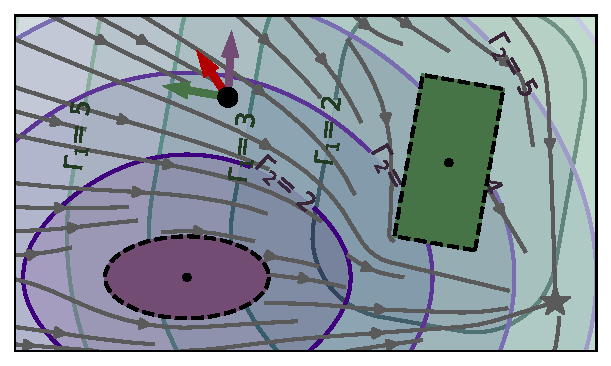
\includegraphics[width=0.5\textwidth]{figures/normal_and_gamma_field_visualization}}
\caption{The $\Gamma$-field for the two obstacles is used to evaluate the averaged normal $\vecs n$ (red arrow). 
Both parameters must ensure the motion follows the avoidance dynamics (gray) towards the attractor (black star) while remaining compliant.}
\label{fig:resultant_normal}
\end{figure}

% There could be cases where the resultant normal is not defined (due to $\vecs{n_i}$'s canceling each other). A solution to this issue is proposed in \ref{limit_cases}.

\subsection{Danger Weight}
Let us define the danger weight function $w(\vecs\xi) \in [0, 1]$ based on the distance to obstacles:
\begin{equation}
  \begin{split}
w(\vecs\xi) =
\max \left(0,  \frac{\Gamma^{\mathrm{crit}} - \Gamma(\vecs\xi)}{\Gamma^{\mathrm{crit}} - 1} \right) \| \vecs n(\vecs \xi) \| \\
\text{with} \quad
\Gamma(\vecs\xi) = \min_{o = 1..N^{\mathrm{obs}}} \Gamma_o(\vecs\xi)
\label{eq:weight_function}
\end{split}
\end{equation}
%% \begin{equation}
%%   %% \Gamma(\vecs\xi) = \min_{o \in \{1, .., N^{\mathrm{obs}} \}} \Gamma_o(\vecs\xi)
%%   \Gamma(\vecs\xi) = \min_{o = 1..N^{\mathrm{obs}}} \Gamma_o(\vecs\xi)
%% \end{equation}
The critical distance $\Gamma^{\mathrm{crit}} \in \mathbb{R}$ defines the distance where the system behaves stiffly towards the obstacle.
Note that $w(\vecs \xi) = 0$ far away from obstacles, and $w(\vecs \xi) = 1$ as it approaches a boundary.

\subsection{Damping Matrix}
While most robotics systems is moving in dimensions $d = 3$, the development in this section can be applied to $d \geq 2$.
% In the following sections, we will consider $N = 3$, which limits the control to a 3-dimensional (Cartesian space in our case). However, the theory presented can easily be extrapolated to work in greater dimensions.
% \subsubsection{Combinaison of the damping matrices}
%% Let us now combine the two matrices:
The desired damping matrix has two goals: it should maintain and follow the desired DS, and at the same time, it has to ensure collision avoidance with obstacles. We define it as a linear combination that achieves these two parts:
\begin{equation}
    \matd D(\vecs\xi) = \left(1 - w(\vecs\xi) \right) {\matd D^{DS}}(\vecs\xi) + w(\vecs\xi)  {\matd D^{\mathrm{obs}}}(\vecs\xi) \label{eq:damping_summation}
\end{equation}
Away from any obstacle, the behavior is fully controlled by $\vecs {D_{DS}}(\vecs\xi)$, and when approaching one, the damping matrix smoothly shifts to also stiffen the control against the obstacle. 
Note that as ${\matd D^{DS}}(\vecs\xi)$ and $\matd {D^{\mathrm{obs}}}(\vecs\xi)$ are positive semi-definite matrices, thus $\matd {D}(\vecs\xi)$ is positive semi-definite, too.


\subsubsection{Dynamic System Following}
The damping matrix, which achieves the dynamical system following $\matd D^{DS}$, is designed as presented in Section~\ref{sec:trad_passive}, following the theory of \cite{kronander2015passive}. $\matd D^{DS}$ has high stiffness in the direction of the desired velocity $\dot{\vecs \xi}$, but is compliant perpendicular to it.

\begin{equation}
  \begin{split}
  s_i^{DS} =
  \begin{cases}
    s^{DS} & i = 1 \\
    w^p s^{\mathrm{obs}} + (1- w^p) s^s & i \geq 2 
  \end{cases} \\
  \text{with} \quad
  w^p = \min \left(1,  \| \vecs n(\vecs \xi) \|^2 + \left(\frac{\Gamma(\vecs \xi) -1}{\Gamma^{\mathrm{crit}} - 1}\right) ^2 \right)
  \end{split}
\end{equation}
where the ds-damping $s^{DS} \in \mathbb{R}$, obstacle-damping $s^{\mathrm{obs}} \in \mathbb{R}$, and the compliant-damping $s^c \in \mathbb{R}$ are user-defined values which define the behavior of the passive-controller.


\subsubsection{Obstacle Repulsion}
Let us define $\vecs q^{DS}_1 (\vecs\xi) = \dot{\vecs \xi} / \lVert \dot{\vecs \xi}\rVert$ the vector aligned to the direction of desired motion and $\vecs q_1^{\mathrm{obs}}(\vecs\xi) =  \vecs n(\vecs\xi) / \lVert\vecs n(\vecs\xi)\rVert$ the vector aligned to the obstacles normal.
In the following, we will omit the dependency of the vectors on $\vecs\xi$ for readability purposes.

% We will now define $\vecs{e_{3,obs}} = \vecs{e_{1,obs}} \times \vecs {e_{1,DS}}$ and $\vecs{e_{2,obs}} = \vecs{e_{3,obs}} \times \vecs {e_{1,obs}}$. This defines the orthonormal basis related to the obstacle, with its second vector being the closest to the DS-following vector $\vecs{e_{1,DS}}$.
\begin{equation}
  \vecs q_2^{\mathrm{obs}} = \frac{\hat{\vecs q}_2^{\mathrm{obs}}}{\| \hat{\vecs q}_2^{\mathrm{obs}} \|}
  \quad
  \hat{\vecs q}_2^{\mathrm{obs}} = \vecs q_1^{DS} - \vecs q_1^{\mathrm{obs}} p \quad  \forall \vecs \xi : | p | < 1
\end{equation}
where the object weight is given as $p = \dotprod{\vecs q_1^{\mathrm{obs}}}{\vecs q_1^{DS}}$
The remaining vectors $\vecs q_i^{\mathrm{obs}}, i = 3, .., N$ are set to be orthonormal. For the case that $| p | = 1$, the second basis $\vecs q_2^{\mathrm{obs}}$ is set to be any orthonormal vector. 
Consequently, we define the damping values to ensure smoothness:
\begin{equation}
  s_i^{\mathrm{obs}} =
  \begin{cases}
    s^{\mathrm{obs}} & i = 1 \\
    (1 -  | p | ) s^c + | p | s^{DS} & i = 2 \\
    s^c & i \geq 3 
  \end{cases}
\end{equation}

\begin{figure}
\centerline{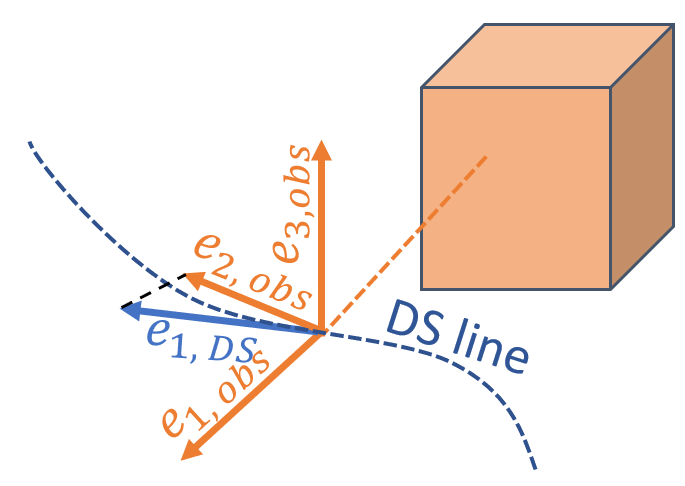
\includegraphics[width=0.5\textwidth]{figures/fig_basis_3D_DS_obs.png}}
\caption{Construction of the basis $\vecs{e_{1,obs}}$, $\vecs{e_{2,obs}}$ and $\vecs{e_{3,obs}}$ in 3D}
\label{fig_basis_3D_DS_obs}
\end{figure}

% Let the matrix $\vecs{Q_{obs}}(\vecs\xi) \in \mathbb{R}^{3\times 3}$ be the matrix whose columns are formed by the orthonormal basis $\vecs {e_{1,obs}}, \vecs {e_{2,obs}}, \vecs{e_{3,obs}}$.\\

% Moreover, let the diagonal matrix $\vecs\Lambda(\vecs\xi) \in \mathbb{R}^{N\times N}$ be the matrix whose diagonal is $\lambda_1(\vecs\xi), \lambda_2(\vecs\xi)$ and $ \lambda_3$. Each eigenvalue corresponds to the damping coefficient along its respective direction given by the vectors.

% Finally we construct $\vecs {D_{obs}}(\vecs\xi)$ as in \eqref{D_matrix_shaping}. Note that the columns of $\vecs Q(\vecs\xi)$ always form an orthonormal basis and that $\lambda_i \geq 0$ $\forall i=1,...,N$. $\vecs D(\vecs\xi)$ is thus a positive semi-definite matrix.

%In the general case, we would have $\lambda_1 = \lambda_{obs}$  corresponding to the damping coefficients associated with moving into an obstacle, $\lambda_2 = \lambda_{DS}$ the tracking stiffness and $\lambda_3 = \lambda_{perp}$ is the coefficient responsible for being compliant in the remaining direction.


% First, we want the damping coefficient $\lambda_2(\vecs\xi)$ to be equal to $\lambda_{DS}$ only when the DS and the obstacle normal are perpendicular. Likewise, we want this coefficient to be equal to $\lambda_{perp}$ when the normal and the DS are collinear. We thus define: 
% \begin{equation}
%     \lambda_2' = \lambda_{perp} \lvert \vecs {e_{1,obs}}^T \vecs {e_{1,DS}} \rvert + \lambda_{DS} (1 - \lvert \vecs {e_{1,obs}}^T \vecs {e_{1,DS}}\rvert)
% \end{equation}
% This also solves the case where $\vecs{e_{1,DS}}$ and $\vecs{e_{2,obs}}$ are perfectly collinear. In this case, the matrix $Q(\xi)$ would become discontinuous, making $D_{obs}$ also discontinuous. This definition of $\lambda_2'$ is designed to converge to the same value as $\lambda_3$, which keeps $D_obs$ always defined.

% The damping coefficient $\lambda_1$ could stay constant. However, we introduce a design that allows for more compliance in XX section.

%% \subsection{Special cases} \label{limit_cases}
%% \subsubsection{Obstacle normal undefined}
%% It could happen that $\vecs n(\vecs \xi)$ is undefined (zero-vector) due to normals of many obstacles canceling each other. To solve this issue, we use smooth step functions. These functions, $H_{a,b}(x)$ and $H_{a,b}^-(x)$, take a value of 0 before $a$ and 1 after $b$, and inversely. They are properly defined in the appendix.
%% As $\lVert \vecs n(\vecs \xi) \rVert \rightarrow 0$, we modify the weight $w$ and make it tend to $0$. This has the effect of smoothly returning to $\vecs D = \vecs{D_{DS}}$, the traditional passive control damping matrix. An implementation is proposed here:  
%% \begin{equation}
%% \label{weight_vanish_norm}
%%     w' = w H_{0, \epsilon}(\lVert \vecs n(\vecs \xi) \rVert)
%% \end{equation}
%% with $\epsilon = 0.01$ chosen in practice.\\
%% Fig.~\ref{fig_smooth_w} shows how this affects the weight function.

%% \begin{figure}
%% \centerline{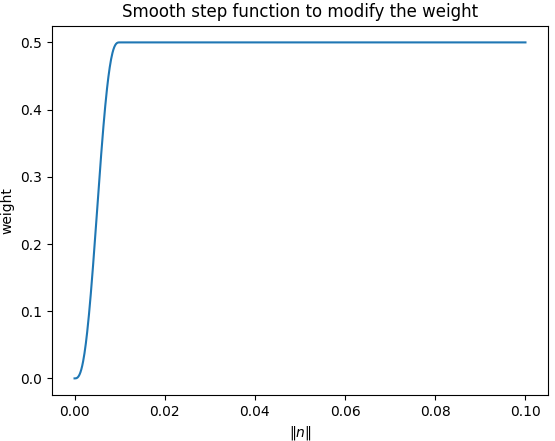
\includegraphics[width=0.5\textwidth]{figures/smooth_step_weight.png}}
%% \caption{Function used to modify the weight when $\lVert \vecs n(\vecs \xi) \rVert \rightarrow 0$. As an example, we took $w = 0.5$.}
%% \label{fig_smooth_w}
%% \end{figure}

\subsection{Damping Only Towards Obstacle} \label{sec:damping_only_toward}
To reject only the disturbances that push the agent against the obstacle and allow compliance in the perpendicular direction away from the obstacle, we have added a new feature. Suppose the robot is currently moving away from the obstacle ($\vecs{\dot\xi}^T \vecs n(\vecs\xi) > 0$). In that case, the value of $\lambda_1$ gets overwritten with $\lambda_{perp}$, the desired damping coefficient for compliance in the orthogonal direction. This ensures that only the disturbances pushing the agent into the obstacle are damped. \\

%% With this feature active, the damping matrix also depends on the velocity. However, as $\vecs{\dot\xi}^T \vecs n(\vecs\xi)$ changes of sign, $\lambda_2$ changes abruptly. This causes $\frac{\partial}{\partial \vecs{\dot\xi}} \vecs D(\vecs{\dot\xi}, \vecs\xi)$ to be infinite at some places, which loses continuity. This can be avoided using again the smooth step functions $H_{a,b}(x)$ and $H_{a,b}^-(x)$. We define,
%% \begin{equation}
%%     \lambda_1' = \lambda_{obs} H_{0,\epsilon}^-(\vecs{\dot\xi}^T \vecs n(\vecs\xi)) + \lambda_{perp} H_{0, \epsilon}(\vecs{\dot\xi}^T \vecs n(\vecs\xi))
%% \end{equation}
%% which is now smoothly defined. We used $\epsilon = 0.01$ in practice.\\

\begin{equation}
  s_1^{DS} =
  \begin{cases}
    s^{DS} & \text{if} \;\; \vecs{\dot \xi}^T \vecs n(\vect \xi) > 0 \\
    0 & \text{otherwise}
  \end{cases}
\end{equation}

Note that in the rest of this work, we will continue referring to $\matd{D}(\vecs{\dot\xi}, \vecs\xi)$ as $\matd D(\vecs\xi)$.


\subsection{Damping Parameter Design}
The damping values are chosen such that $s^{\mathrm{obs}}$ is high to ensure a big damping towards the obstacle. $s^{DS}$ should have a medium-high value to ensure motion in the desired direction. And finally, $s^{c}$ is chosen smaller to allow compliance in all other directions. Thus, we have:
\begin{equation}
s^{\mathrm{obs}} > s^{DS} \gg s^{c} > 0
\end{equation}

% here the subsection with proof of lukas
\subsection{Passivity Analysis}
\subsection{Passivity Analysis}
The stability analysis of the system gives information about the region of stability of the proposed controller. We analyze passivity by observing the evolution of the kinetic energy of the system, given as:
\begin{equation}
	W(\vecs \xi, \vecs{\dot \xi}) = \frac{1}{2}  \dot{\vecs{\xi}}^T \matd{M}(\vecs \xi) \dot{\vecs{\xi}} \label{eq:energy_system}
\end{equation}

\begin{lemma} \label{lemma:passivity}
  % Let $\vect f(\vecs \xi)$ be the desired velocity with bounded magnitude, i.e., $\| \vect f(\xi) \| < \infty, \forall \xi \in \mathbb{R}^N$.
   Let us assume a robotic system as described in \eqref{eq:robot_dynamics} is controlled using \eqref{eq:control_command} using the damping matrix $\matd D(\vecs \xi)$ given in \eqref{eq:damping_summation} with damping values $s_d = 1, d = 1 .. N$.
   The system is passive with respect to the input-output pair $\vecs \xi_e$, $\vecs{\dot \xi}$ when exceeding the desired velocity $\vect f(\vecs \xi)$ , i.e., $\dot{W} \leq \vecs{\dot \xi}^T \vecs \tau^e, \; \forall \vecs \xi \in \mathbb{R}^N: \| \vecs{\dot \xi} \| \geq \| \vect f(\vecs \xi) \|$ and the storage function being the kinetic energy $W \in \mathbb{R}_{>0}$ given in \eqref{eq:energy_system}
\end{lemma}

\begin{proof}
The time derivative of storage function $W$ can be evaluated as:
\begin{align}
  % \begin{split}
	& \dot W(\vecs \xi, \vecs{\dot \xi}) =
    \vecs{\dot \xi}^T \matd M(\vecs \xi) \vecs{\ddot \xi}  + \frac{1}{2} \vecs{\dot \xi}^T \dot{\matd M}(\vecs \xi) \vecs{\dot \xi}  \nonumber \\
  &= \frac{1}{2} \vecs{\dot \xi}^T \left( \dot{\matd M}(\vecs \xi) - 2 \matd C(\vecs \xi) \right) \dot{\vecs \xi} - \vecs{\dot \xi}^T \matd{D}(\vecs \xi) \left(\vecs{\dot \xi} - \vect f(\vecs \xi) \right) + \vecs{\dot \xi}^T \vecs \tau^e \nonumber \\
  &= - \vecs{\dot \xi}^T \matd{D}(\vecs \xi) \left( \vecs{\dot\xi} - \mathbf{f}(\vecs \xi) \right) + \vecs{\dot\xi}^T \vecs{\tau}^e
  % \end{split}
\end{align}
where the second order dynamics $\vecs{\ddot \xi}$ are evaluated according to the rigid body dynamics defined in \eqref{eq:robot_dynamics}. Furthermore, $\dot{\matd M} - 2 \matd C$ is skew-symmetric for any physical system; hence, the corresponding summand is zero.

% \subsubsection{Stability with Uniform Damping}
Let us investigate the region where the passivity holds. Since in the Lemma, we assumed all damping values being equal to one, we have:
\begin{equation}
	\matd{D}({\vecs \xi}) = \matd{Q}({\vecs \xi}) \matd{S} ({\vecs \xi}) \matd{Q}({\vecs \xi})^{-1}= \matd{Q}({\vecs \xi}) \matd{I} \matd{Q}({\vecs \xi})^{-1} = \matd{I}
\end{equation}
where $\matd{I} \in \mathbb{R}^{N \times N}$ is the identity matrix.

It follows that the system is passive with respect to the input, the external force $\tau^e$, and the output, the velocity $\dot {\vecs \xi}$, as long as:
\begin{equation}
	\dot{\boldsymbol {\vecs \xi}}^T \matd{D}({\vecs \xi}) \left(\dot{\boldsymbol {\vecs \xi}} - \boldsymbol{f}(\boldsymbol {\vecs \xi}) \right) = 
    \dot{{\vecs \xi}} ^ T \Delta \vect{f}  \geq 0 
 \; , \quad
 \Delta \vect{f} = \dot{{\vecs \xi}} - \vect{f}({\vecs \xi})
 \label{eq:passivity_condition}
\end{equation}

On the border of this region, the two vectors $\Delta \vect{f}$ and $\dot{{\vecs \xi}}$ are orthogonal.
Hence, using Thale's theorem, this region can be interpreted as a circle in velocity-space with radius $\| \vect{f} ({\vecs \xi}) \| / 2$ and center $\vect{f}({\vecs \xi}) / 2$, see Figure~\ref{fig:passivity_analysis}.

\begin{figure}[thb]
	\centering
	% \includesvg[width=0.7\columnwidth]{figures/passivity_analysis.svg}
	\ifthesis
    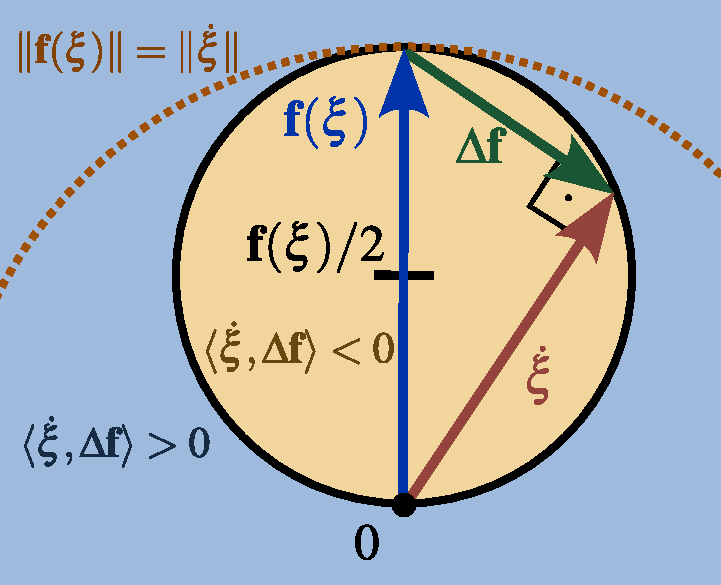
\includegraphics[width=0.7\columnwidth]{figures/passivity_analysis}
	\else
    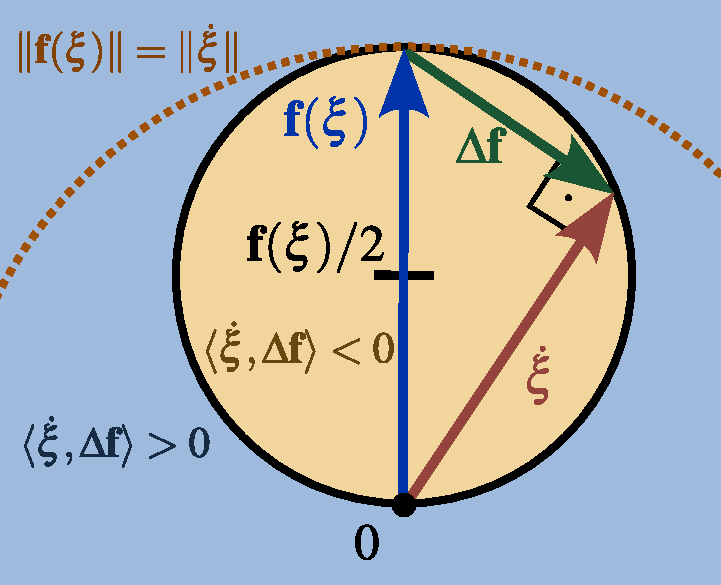
\includegraphics[width=.7\columnwidth]{figures/passivity_analysis}
	\fi
	\caption{Analyzing the system in velocity-space, yields that the system is passive if it has a velocity $\dot{\vecs \xi}$ larger than the desired velocity $\vect f(\vecs \xi)$, i.e., outside the dashed circle.
    However, the system can be non-passive for small velocities when  $\dotprod{\dot{\vecs \xi}}{\Delta \vect f} < 0$ (yellow circle).}
	\label{fig:passivity_analysis}
\end{figure}

Moreover, the system is passive as long as the observed velocity $\dot{{\vecs \xi}}$ is outside the circular-red region, which is a subset of the region where the magnitude of the observed velocity is smaller than the desired velocity $\vect {f}({\vecs \xi})$, i.e.,
\begin{equation}
	\dot W({\vecs \xi}, \dot{{\vecs \xi}}) \leq \dot{{\vecs \xi}}^T \vecs \tau^e
 \quad \forall {\vecs \xi} : \| \dot{{\vecs \xi}} \| \geq\| \vect{f}({\vecs \xi}) \| 
\end{equation}

\end{proof}

As in the orange region, the system is not passive; the storage function $W$ could increase, and hence, the velocity $\dot {\vecs \xi}$ increases non-passively. This behavior is not unexpected, as the controller is designed to approach the desired dynamics $\vect{f}({\vecs \xi})$. Hence, as long as the desired velocity is not reached, the kinetic energy increases even with no force input $\vecs \tau^e$. However, as soon as the system velocity $\dot{\vecs \xi}$ exceeds the desired velocity $\vect f(\vecs \xi)$, the system behaves passively. We can use this to ensure the stability of the system:

\begin{theorem}  \label{theorem:passivity}
  Let $\vect f(\vecs \xi)$ is the desired velocity with bounded magnitude, i.e., $\| \vect f(\vecs \xi) \| < v^{\mathrm{max}}, \forall \vecs \xi \in \mathbb{R}^N$.
   The closed loop system \eqref{eq:robot_dynamics} using the controller from \eqref{eq:control_command} and the damping matrix $\matd D(\vecs \xi)$ given in \eqref{eq:damping_summation} is bounded-input, bounded-output (BIBO) stable with respect to the input disturbance force $\vect \tau^e$, and output the velocity $\dot{\vecs \xi}$ for all times $T = 0, \, .., \, \infty$.
\end{theorem}
 
\begin{proof}
% From Lemma~\ref{lemma:passivity}, the system is passive when the magnitude of the velocity is larger than the dynamics, i.e. $\| \dot{\vecs \xi} \| > \|\vect f(\vecs \xi) \|$, the orange circle in Figure~\ref{fig:passivity_analysis}.
% The system is not passive inside this region, and the velocity $\dot {\vecs \xi}$ can increase. However, the velocity increase is limited to staying below $\| \vect f({\vecs \xi}) \|$ before the system enters the region where it is passive. Hence, the control cannot introduce unexpected energy.
% It follows that the system has a bounded output as long as the desired velocity $\vecs{f}({\vecs \xi})$ is stable and the input $\int_{0}^T \dot{{\vecs \xi}}^T \vecs \tau^e dt$ is bounded. 

To ensure BIBO stability, let us analyze the integral of the impulse of the response for the external force $\vecs \tau^e$: 
\begin{equation}
	\begin{split}
	  \int_{0}^{T} \left\| \dot{\vecs \xi} \right\| \; dt 
	  & = \int_{t \notin \mathcal{T}_n} \left\| \dot {\vecs \xi} \right\|  \, dt + \int_{t \in  \mathcal{T}_n} \left\| \dot {\vecs \xi} \right\| \;  dt \\ 
	  % & = \int_{t : \| \dot{\vecs \xi} \| > \| \vect f(\vecs \xi) \|} \dot {\vecs \xi} \, dt + \int_{t : \| \dot{\vecs \xi} \| \leq \| \vect f(\vecs \xi) \|} \dot {\vecs \xi} \;  dt \\ 
	  % & \leq \int_{t \notin \mathcal{T}_n} \left| \dot {\vecs \xi} \right| dt + v^{\mathrm{max}}  T_n \\ 
	  & \leq K_p + v^{\mathrm{max}} T_n
\end{split}
\label{eq:bibo_velocity}
\end{equation}
where $\mathcal{T}_n$ denotes the set of time instances where the system is not shown to be passive (Fig.~\ref{fig:passivity_analysis}), specifically $\| \dot{\vecs \xi} \| \leq \| \vecs f (\vecs \xi) \|$, and $T_n \in \mathbb{R}_{\geq 0}$ is the total duration which the system spends in this region. Additionally, from passivity in the inner region, the system is bounded by a constant $K_p \in \mathbb{R}_{\geq 0}$.
Hence, the impulse response is bounded, and the system is BIBO stable.

% \subsubsection{Stability with General Damping}
However, from \eqref{eq:damping_summation}, we know that a general damping matrix $\matd{S}(\vecs \xi)$ can have non-uniform diagonal values. This is analyzed by introducing the coordinate transfers:
\begin{equation}
	\vecs{\bar{v}} = \sqrt{\matd{S}({\vecs \xi})} \matd{Q}({\vecs \xi})^{-1} \dot{{\vecs \xi}}
	\;\; \text{and} \;\;
	\bar{\Delta \vect f} = \sqrt{\matd{S}({\vecs \xi})} \matd{Q}({\vecs \xi})^{-1} \Delta \vect{f}
\end{equation}
where the square root of the diagonal matrix $\matd{S}({\vecs \xi})$ is taken element-wise.

The transfer is then used to rewrite \eqref{eq:passivity_condition} as:
\begin{equation}
\dot{\vecs \xi}^T \matd{D}({\vecs \xi}) \Delta \vect{f} = \vecs{\dot \xi}^T \matd{Q}({\vecs \xi}) \matd{S}({\vecs \xi}) \matd{Q}({\vecs \xi})^{-1} \Delta \vect{f} = \vecs{\bar v}^T \bar{\Delta \vect f}
\end{equation}

Hence, the BIBO analysis of \eqref{eq:bibo_velocity} applied to the transformed system results as:
\begin{equation}
\begin{split}
	  & \int_{0}^{T} \left\| \vecs{\bar v} \right\| \; dt   
	   = \int_{t \notin \bar{\mathcal{T}}_n} \left\| \vecs{\bar v} \right\|  \, dt + \int_{t \in  \bar{\mathcal{T}}_n} \left\| \vecs{\bar v} \right\| \;  dt  \\ 
   & < K_p + v^{\mathrm{max}} \bar T_n 
   {\max{\Bigl(\text{eig}\bigl(\mathcal{D} \bigr) \Bigr)}} 
   / {\min{\Bigl(\text{eig}\bigl(\mathcal{D} \bigr) \Bigr)}}
\end{split}
\end{equation}
where $\bar{\mathcal{T}}_n$ denotes the region where the transformed system $\vecs{\bar v}$ is not shown to be passive, i.e. $\| \vecs{\bar v} \| \leq \| \bar{\Delta \vect f} \|$, and $\bar T_n \in \mathbb{R}_{\geq 0}$ the corresponding time. Additionally, $\min{(\text{eig}(\mathcal{D}))}$ and $\max{(\text{eig}(\mathcal{D}))}$ are the smallest and largest eigenvalue of the damping matrix $\matd{D}$ respectively.

Hence, since the transformed system with velocity $\vect {\bar v}$ is BIBO stable, the original system with velocity $\dot{\vecs \xi}$ is BIBO stable, too, as long as it is a continuous, finite transform. 
\end{proof}
% The analysis described in Fig.~\ref{fig:passivity_analysis} can hence be applied in the transformed space, too. 

For an orthogonal decomposition matrix $\matd{Q}(\boldsymbol{{\vecs \xi}})$, the region of non-passivity is an ellipse where the direction of the axes points along column vectors of $\matd{Q}({\vecs \xi})$, and the corresponding axes lengths are the diagonal elements of $\| \mathbf{f}({\vecs \xi})^T \sqrt{\matd{S}({\vecs \xi})}\| / 2 \sqrt{\matd{S}({\vecs \xi})}^{(-1)}$. 
If the ratio of the first damping value to the other axis $i \geq 2$ is large, i.e., $s_1 / s_i \gg 1$, it can lead to non-passivity even though the velocity $\dot{\vecs \xi}$ is already larger (but not pointing in the correct direction) than the desired velocity. However, the non-passive region is still bounded \iflong (Fig.\ref{fig:passivity_analysis_skew}) \fi.
This proof holds for any basis $\matd{Q}$ which is not singular. However, the controller must be carefully chosen to ensure that the speed up is limited when the basis is close to singular, for example, by limiting the relative difference of the stretching vectors. Furthermore, as stable behavior is ensured for a general shape of a damping matrix $\matd{D}(\vecs \xi)$, the global stability proof extends to any positive definite damping matrix matrices.

Since the damping matrix $\matd D(\vecs \xi)$ changes dynamically, a change in the environment can move the system outside of the passive region. However, there exists always a finite maximum velocity, at which the system is ensured to be passive.

\iflong
\begin{figure}[htbp]
    \centering
    \begin{subfigure}{0.49\columnwidth}
      \centerline{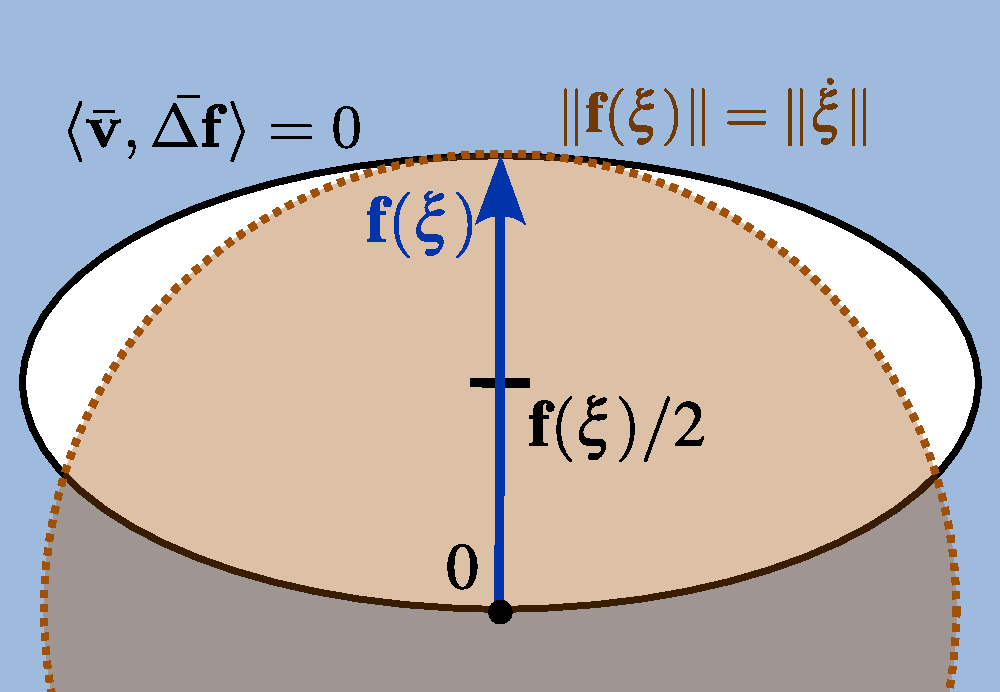
\includegraphics[width=\textwidth]{figures/passivity_analysis_wide}}
	  \caption{$\matd{S}_1^f > \matd{S}_2^f$, $w \approx 0$}
	  \label{fig:passivity_analysis_wide}
    \end{subfigure}\hfill%
    \begin{subfigure}{0.49\columnwidth}
    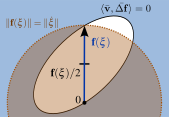
\includegraphics[width=\textwidth]{figures/passivity_analysis_skew}
	\caption{$\dotprod{\vect f(\vecs \xi)}{\vect q_1} \neq \| \vect f(\vecs \xi)\| \; \| \vect q_2\| $ }
      \label{fig:passivity_analysis_skew}
    \end{subfigure}
	\caption{
		The stability is ensured even if the controller can temporarily accelerate the system  to reach a velocity $\dot{\vecs \xi}$, which is faster than the desired velocity $\vect f(\vecs \xi)$ (white region).
		This happens when the eigenvalues of the damping matrix $\matd{D}(\vecs \xi)$ are not uniform (a) or the stretching vectors $\vect q_1$ and $\vect q_2$ are not orthogonal (b). 
	In both cases, the region of non-passivity is elliptical (black circle).
}
	\label{fig:passivity_analysis_varied}
\end{figure}
\fi


% Note, that in the case of $\langle e_2, e_n \rangle \neq 0$ the choice of $e_2$ does not matter as the corresponding  weight from \eqref{eq:eig2_weight} is $w_2 = 0$, hence it $\lambda_2 = \lambda$, as all eigenvalues.


\section{Collision Avoidance} \label{sec:collision_avoidance}
\subsection{Inertia Drift}
Let us assume that have strong damping in the direction of the obstacle, i.e., $s^{\mathrm{obs}} / m_i \gg 1$, where $m_i$ with $i = 1, .., N$ represent the eigenvalues of the mass matrix $\matd{M}$. 


\subsection{Disturbance Repulsion}
Let us assume a disturbance impact at time $t_0$, which results in the robot having an impact velocity of $\vecs{\dot \xi} = \vect v^I$, which is pointing towards the obstacle. The impact velocity is much larger than the robot's initial velocity. Thus the latter is neglected, and the obstacle is approximated as locally flat and the velocity locally constant (see Fig.~\ref{fig:collision_avoidance}). Furthermore, we assume to be close to the robot, i.e., $\Gamma(\vecs \xi) \approx 1$, hence the $w(\vecs \xi) \approx 1$, and the stiffness in the direction of the obstacle is approximated as $s^{\mathrm{obs}}$.
No further impact forces are applied after the initial impact is absorbed. The Coriolis effect is neglected in the short time frame.

The velocity with the controller can be analyzed as follows:
\begin{equation}
    \vecs{\dot \xi} = \int \vecs{\ddot \xi} \, dt = \int \matd{D} \matd{M}^{-1} \left( \vecs{\dot \xi} - \vecs f(\vecs \xi) \right) \, dt
\end{equation}

Let us analyze when the decoupled velocity along the normal reaches zero:
\begin{equation}
    \vecs{\dot \xi} = \int \frac{s^{\mathrm{obs}}}{m} \vecs{\dot \xi} \, dt = \frac{s^{\mathrm{obs}}}{m} \vecs{\xi} + \| \vecs v^I \| \label{eq:velocity_with_control}
\end{equation}
It can be seen that the velocity along the normal reaches zero at position, i.e., 
\begin{equation}
    \vecs{\xi} = \| \vecs v^I \| {m} / {s^{\mathrm{obs}}} 
    \quad \Rightarrow \quad
    \| \vecs{\dot \xi} \| =
\end{equation}

\begin{lemma}

\end{lemma}

\begin{proof}
The statement follows directly from \eqref{eq:velocity_with_control}.
\end{proof}

\subsection{Disturbance Repulsion with Force Limit}
Robotic systems have a maximum force that can be exerted based on the motors and their geometry, $\tau_c^{\mathrm{max}} \in \mathbb{R}_{>0}$. Note that this maximum might be state dependent.

Let  us assume strong damping concerning the maximum force, i.e., $s^{\mathrm{obs}} / \tau_c^{\mathrm{max}} \gg 1$, hence we can assume that the magnitude of the obstacle repulsive force is equal to the maximum force close to the obstacle. Hence, the maximum disturbance.

\subsection{Practical Considerations}

\begin{figure}
\centering
\begin{subfigure}{0.99\columnwidth}
  \centerline{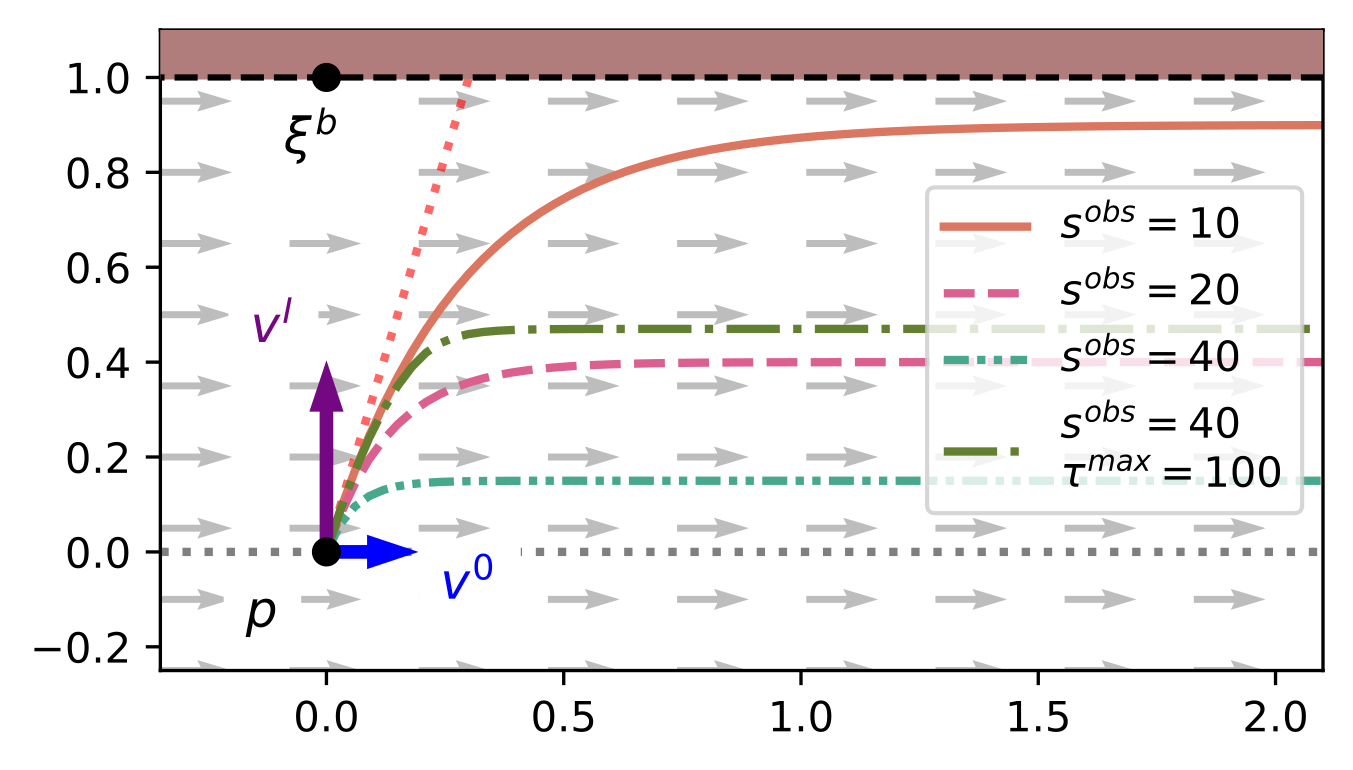
\includegraphics[width=\textwidth]{figures/parallel_avoidance_obstacle}}
  \caption{Traditional passive control}
\end{subfigure}
% \begin{subfigure}{0.5\columnwidth}
%   \centerline{\includegraphics[width=\textwidth]{}}
%   \caption{Obstacle aware passive control}
% \end{subfigure}
\caption{Comparison of the two control methods}
\label{fig:collision_avoidance}
\end{figure}


% continue here, noisy graphs ready to run

\section{Evaluation}  \label{sec:evaluation}
\subsection{Qualitative Comparison} \label{sec:qual_comp}
The control law presented was tested in simulation in Python. The state space is the Cartesian coordinates $xy$ in 2D and $xyz$ in 3D. In practice, the damping matrix $\matd D(\vecs\xi)$ and the control command $\vecs {\tau_c}$ are recomputed at each time step.\\

Let us compare traditional passive interaction control and the presented method (Fig.~\ref{fig_diff_obs_pass}). On the setup, the same disturbance is applied to both systems simultaneously. One can already see the robot equipped with traditional passive control (left) penetrates the obstacle, while ours (right) successfully damps the disturbance.

\begin{figure}
\centering
\begin{subfigure}{0.8\columnwidth}
  \centerline{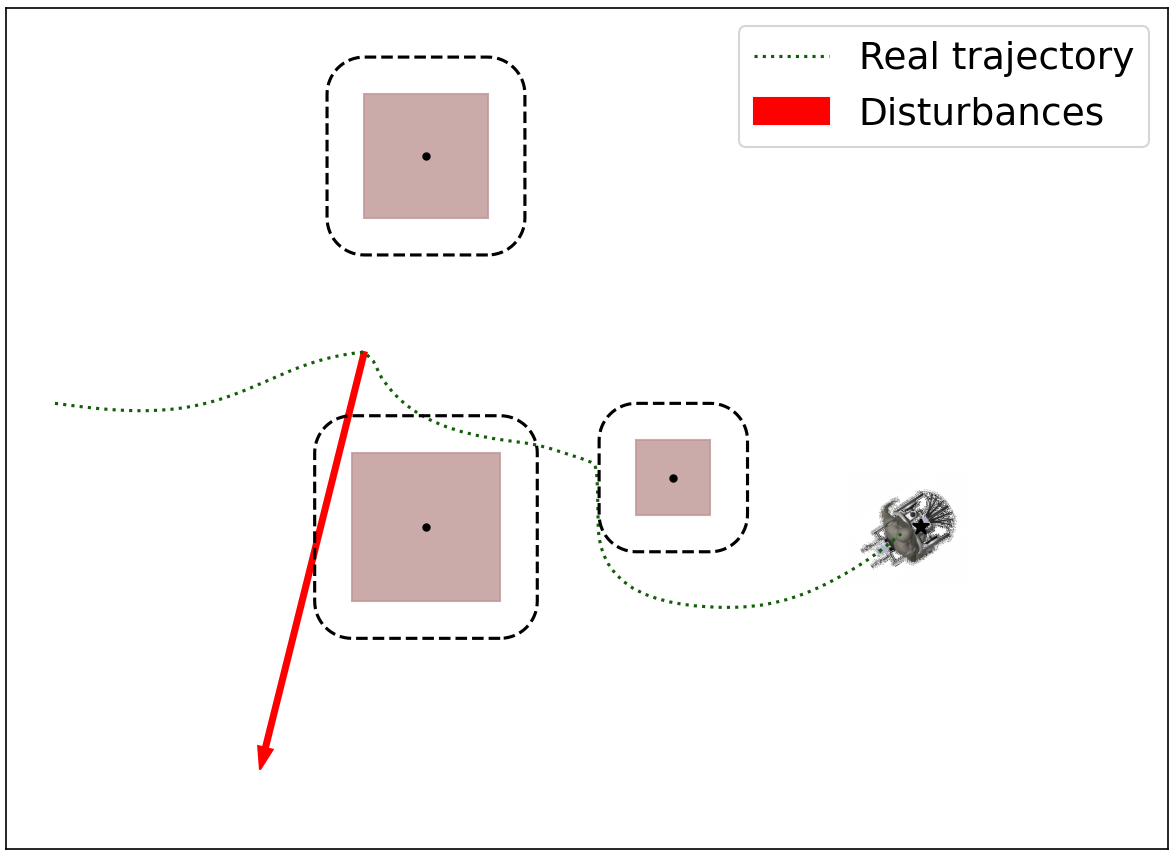
\includegraphics[width=\textwidth]{figures/run_without_pass.png}}
  \caption{Traditional passive control}
\end{subfigure}
\begin{subfigure}{0.8\columnwidth}
  \centerline{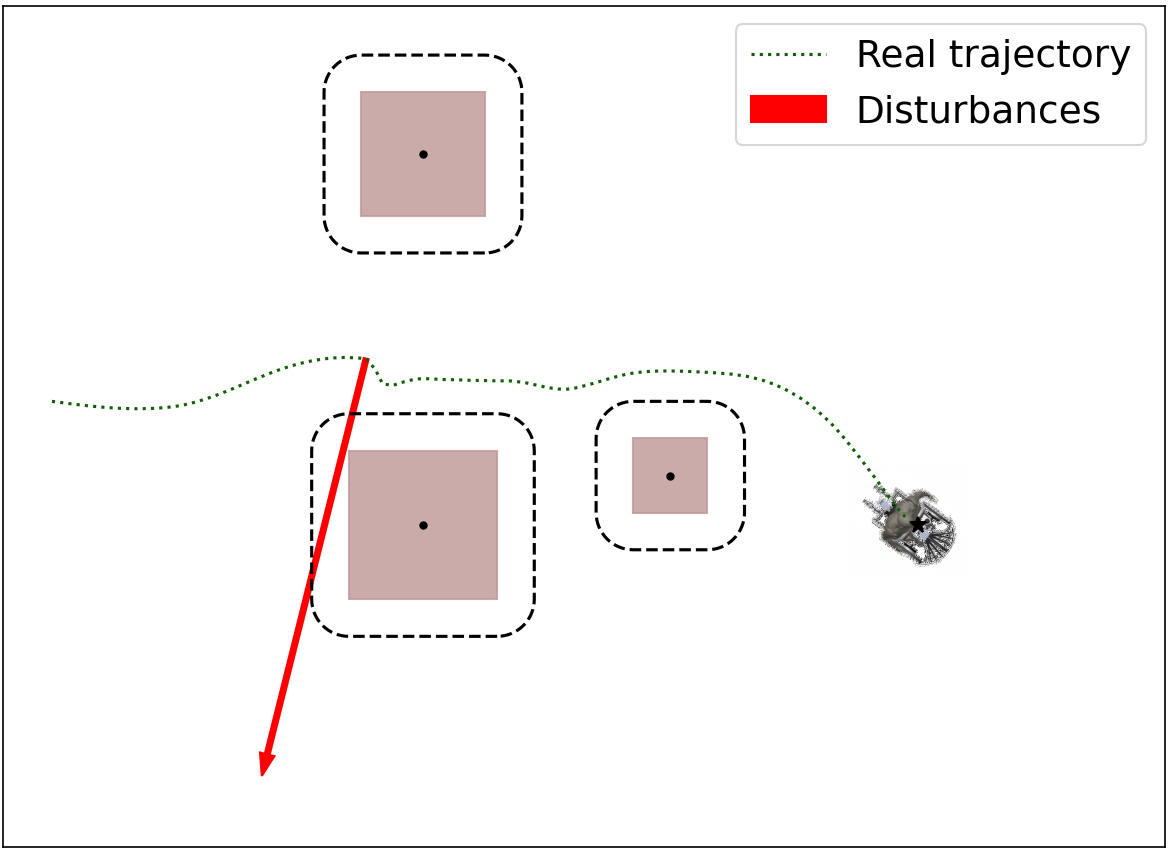
\includegraphics[width=\textwidth]{figures/run_with_pass.png}}
  \caption{Obstacle aware passive control}
\end{subfigure}
\caption{Comparison of the two control methods}
\label{fig:diff_obs_pass}
\end{figure}

\subsection{Comparison to Reference Trajectory}
We will now look at the performance of our controller in different scenarios. Fig.~\ref{fig_run_with_obs} shows a simulation with 3 obstacles. The red arrows represent manually applied disturbances. The ideal trajectory is also displayed (perfect DS tracking, not subjected to real dynamics). Based on this simulation, we can observe the robots' behavior in different scenarios.

The first disturbance (A) pushed the robot in a direction perpendicular to the desired motion. Since we want compliance in this direction and the robot is far from any obstacle, it deviates greatly from its previous trajectory. It continues its path to the attractor on another DS line.

Another disturbance (B) pushed the robot toward the obstacle and was successfully damped, avoiding the collision.

A disturbance (C) pushed the robot away from an obstacle. The control algorithm is made such that when moving away from an obstacle, disturbances are not damped, and the robot shows compliant behavior. 

The last disturbance (D) was applied along the direction of motion. As the desired behavior is stiff in this direction, the robot almost kept the same speed and continued toward the attractor. \\

\begin{figure}
\centerline{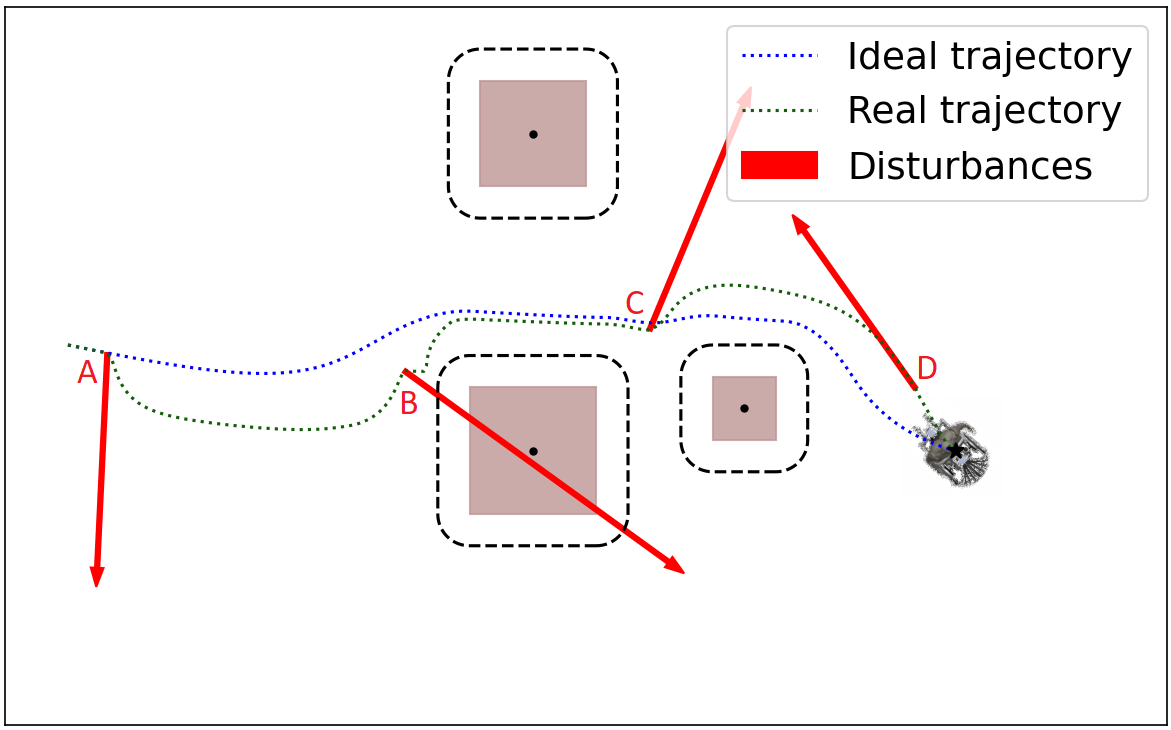
\includegraphics[width=0.5\textwidth]{figures/run_with_obs.png}}
\caption{Simulation with a complex environment and disturbances applied to the robot}
\label{fig_run_with_obs}
\end{figure}

Furthermore, in Fig.~\ref{fig_run_damped_towards}, one can observe the feature described in Section~\ref{sec:damping_only_toward}, that only damps the disturbance towards the obstacle.
The first disturbance is highly damped, while the second is much less. This feature provides a natural behavior of moving away from obstacles, improving the margin of impenetrability. 

\subsection{Noise analysis}
Gaussian noise was added to the simulation to assert the control law's robustness. We added two types of noise, noise on the position measurements and noise on the velocity measurements. 

The experiment is done on a simple setup with one obstacle. The noise added has a mean of $0$, and the standard deviation is increasing linearly from $0.0$ to $0.7m$ for position and $0.0$ to $7.0 \frac{m}{s}$ for velocity measurements. For each noise level, the simulation was run 10 times. The output variable is the smallest distance of the agent from the obstacle during the simulation. This metric was chosen to observe how the noise could lead to a crash in the obstacle. 

For the noise acting on the position measurement, the controller presents good rejection for a small noise variance. As it increases, the robot's behavior quickly worsens (Fig.~\ref{fig_pos_noise}). The robot penetrates the obstacle for noises of standard deviation $ > 0.4 m$. An example of a run with $\sigma_{noise} = 0.7 m$ is shown in Fig.~\ref{fig_pos_noise_0_7}.

\begin{figure}
\centerline{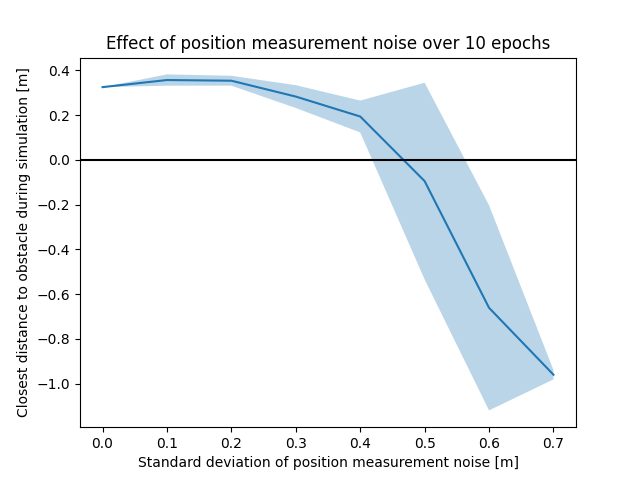
\includegraphics[width=0.5\textwidth]{figures/noise_pos_v2.png}}
\caption{Noise on the position measurements (shaded region are within one standard deviation from the mean)}
\label{fig_pos_noise}
\end{figure}

\begin{figure}
\centerline{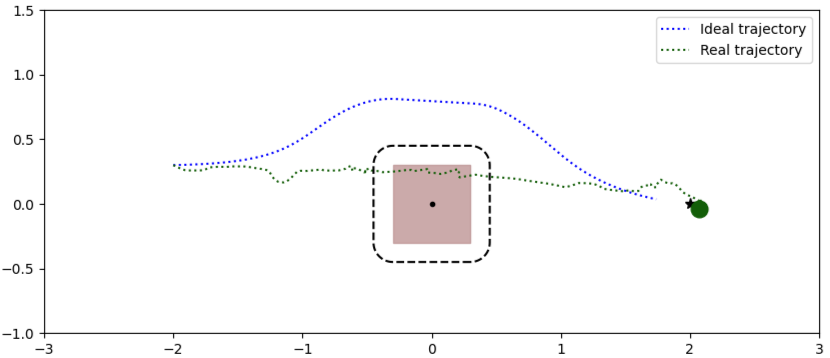
\includegraphics[width=0.5\textwidth]{figures/noise_effect_0_7.png}}
\caption{Noise on the position measurement with a standard deviation of 0.7 $m$ (with ideal trajectory displayed)}
\label{fig_pos_noise_0_7}
\end{figure}

The obstacle was never penetrated for the velocity measurement noise, asserting the robustness of the control for this type of noise (Fig.~\ref{fig_vel_noise}). Fig.~\ref{fig_2_vel_noise} provides an image of the simulation with big noise standard deviation ($4.0 \frac{m}{s}$). Thanks to the feature presented in Section~\ref{sec:damping_only_toward} (damping only toward the obstacle), the robot has even the tendency to drift away from the obstacle, increasing the safety margin.

\begin{figure}
\centerline{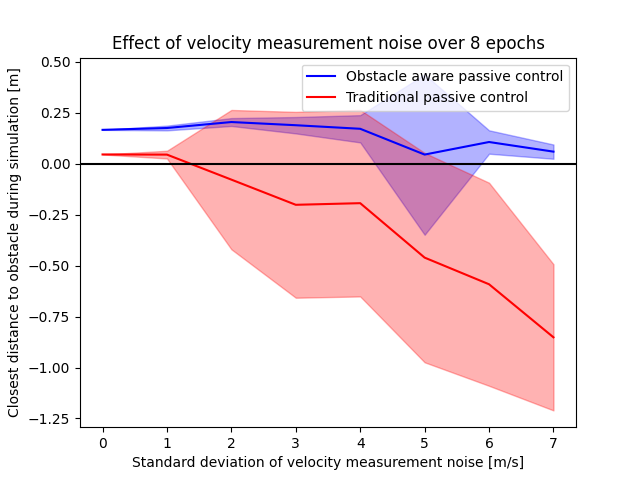
\includegraphics[width=0.5\textwidth]{figures/vel_noise_0.png}}
\caption{ NOT this one - Noise on the velocity measurements (shaded regions are within one standard deviation from the mean)}
\label{fig_vel_noise}
\end{figure}

\begin{figure}
\centerline{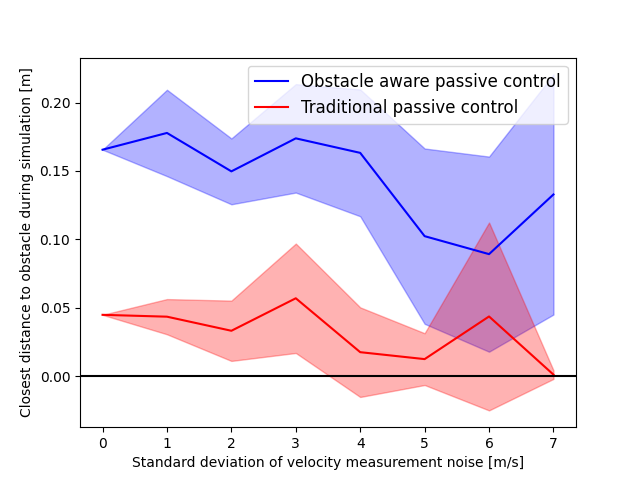
\includegraphics[width=0.5\textwidth]{figures/vel_noise_cliped_0.png}}
\caption{Noise on the velocity measurements (shaded regions are within one standard deviation from the mean) - NEW FINAL }
\label{fig_vel_noise}
\end{figure}

\begin{figure}
\centerline{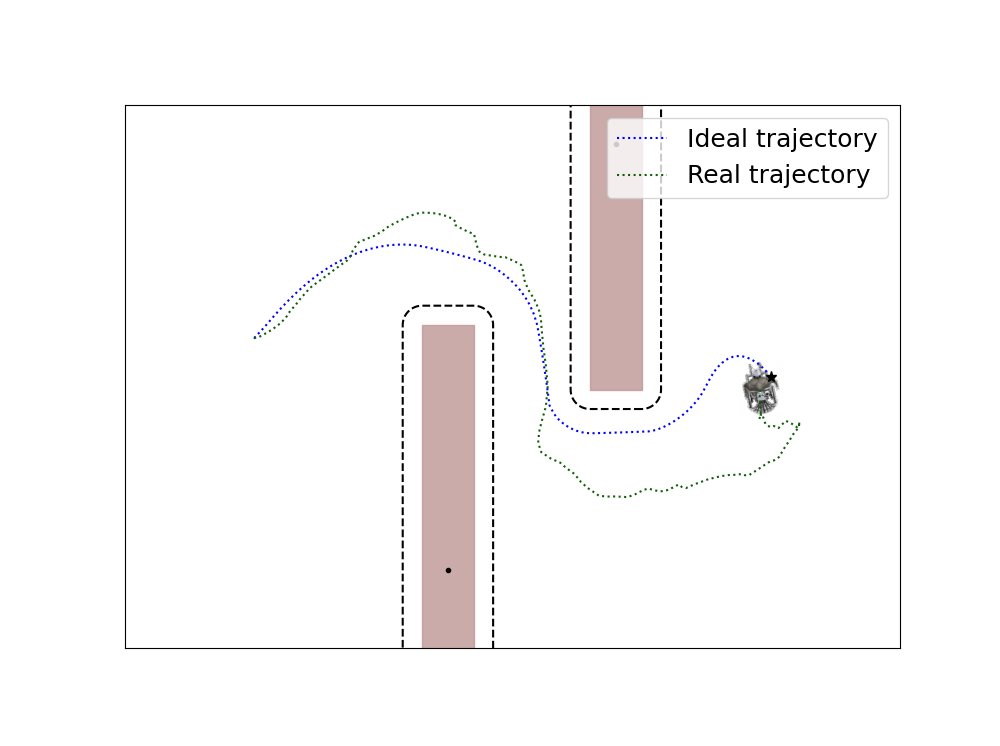
\includegraphics[width=0.5\textwidth]{figures/noise_setup.png}}
\caption{setup}
\label{fig_vel_noise}
\end{figure}


\begin{figure}
\centerline{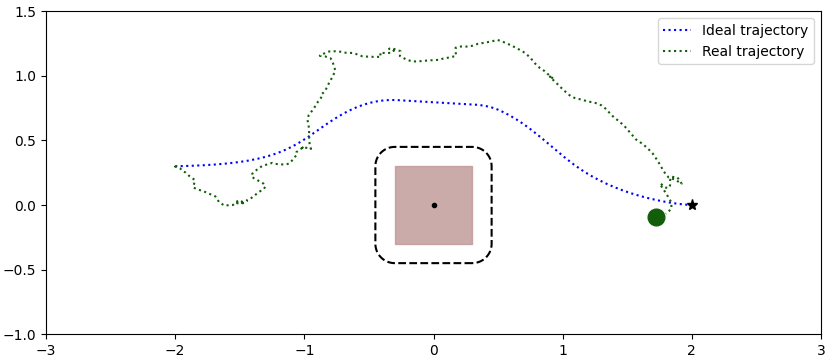
\includegraphics[width=\columnwidth]{figures/vel_noise_4.0.png}}
\caption{A simulation with noise on the velocity measurement with a standard deviation of $4.0 \frac{m}{s}$  (with ideal trajectory displayed)}
\label{fig_2_vel_noise}
\end{figure}
 
\section{Discussion}
Overall, the simulated robot shows pleasing results. It has good tracking performances, compliance in the direction perpendicular to the motion, and great damping of the disturbances towards obstacles.
Away from obstacles, the controller presented shows similar behavior as the one in \cite{kronander2015passive}. When approaching one obstacle, the control gets stiffer to avoid collisions without losing its tracking properties. This makes the proposed controller a suitable option to cumulate good tracking and safety regarding obstacle penetration.

\subsection{Applicability Approach}
Note, that the theoretical analysis from Theorem~\ref{theorem:passivity}, indicates passivity for any velocity-bounded, uniquely damped system. As a result, work such as the damping-based controller in  \cite{kronander2015passive} does not require an energy tank anymore.
Conversely, if the impedance controller has a proportional $\mathcal{K}$, the adaptive proportional term might induce instabilities even for stable desired dynamics as pointed out in \cite{ferraguti2013tank, kronander2016stability}.

\begin{figure}
\centering
\begin{subfigure}{1\columnwidth}
\centerline{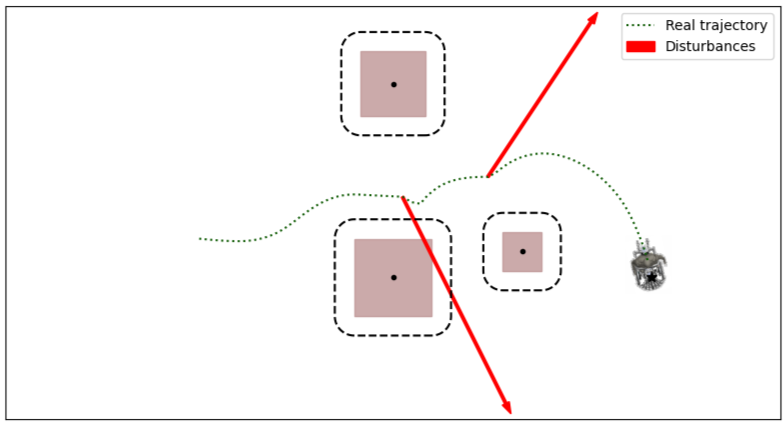
\includegraphics[width=\textwidth]{figures/first_meth.png}}
  \caption{First method (presented)}
\end{subfigure}
\caption{Little disturbance is observed when 3}
\label{fig_all_3_meth}
\end{figure}


% \appendix
% \section{Appendix}
% \label{Appendix}


\renewcommand*{\bibfont}{\footnotesize}
\printbibliography

\end{document}
